\documentclass[12pt]{article} % Tamaño de letra
\usepackage[utf8]{inputenc} % Simbolo utf8
\usepackage[light]{antpolt} % Tipo de letra
\usepackage[T1]{fontenc}
\usepackage[spanish]{babel} % Español 
\usepackage[dvipsnames]{xcolor} % Paquete de colores
\usepackage{amsmath} % Paquete de simbolos matematicos
\usepackage{halloweenmath} % Paquete de Halloween
\usepackage{amssymb} % therefore 
\usepackage{amsfonts}  % Alinear
\usepackage{mathtools} 
\usepackage{hyperref} % Hiperreferencias
\usepackage{xurl} % Romper url largos en más líneas
\usepackage{graphicx}
\usepackage{caption} % Paquete para personalizar las captions
\usepackage{tikz} % Dibujos arreglo
\usepackage{graphics}
\usepackage{wrapfig}
\usepackage{subfig}
\usepackage{listings} % Código
\usepackage[shortlabels]{enumitem}
\usepackage{bbm}
\usepackage{multirow, array} % para las tablas
\usepackage{float}
\usepackage{color}
\usepackage{tabularray}
\usepackage{fancyhdr}
\usepackage{pifont}%Simbolos especiales.
\usepackage{fancybox}%Para crear cajas (Notas).
\usepackage[margin=1in]{geometry}
\usepackage[margin=1.1in]{caption}
\pagestyle{fancy}
\fancypagestyle{plain}{
\fancyhf{}\fancyhead[L]{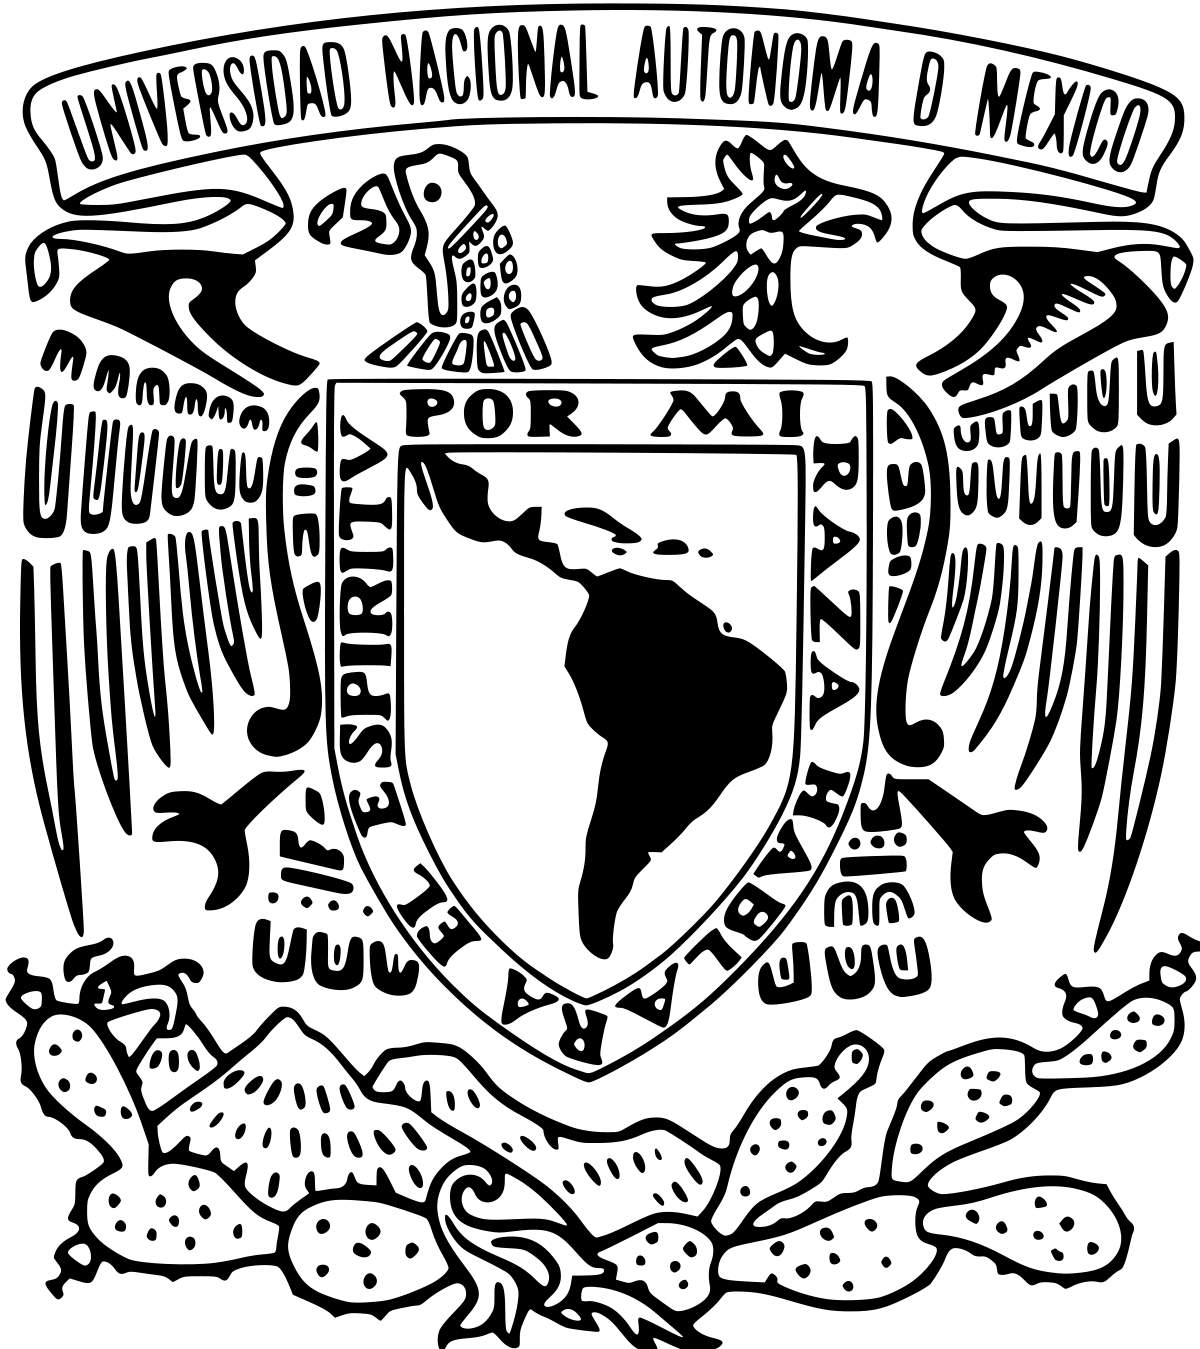
\includegraphics[height=0.5in]{unam.png}}
\fancyhead[R]{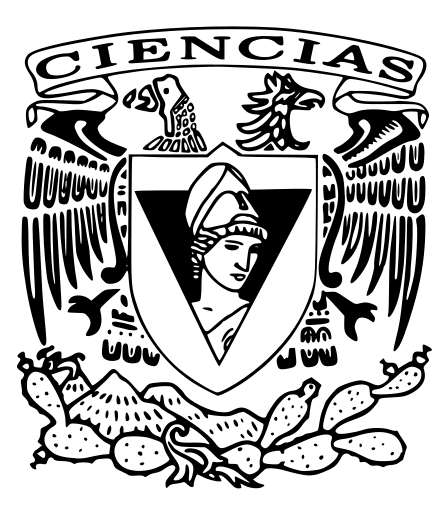
\includegraphics[height=0.5in]{ciencias.png}}
}

%----------[ Declaración Respuesta ]-----------
\usepackage{framed,xcolor} % Color de repuesta

\newenvironment{respuesta}{
    \definecolor{shadecolor}{RGB}{236,236,228}
    \begin{snugshade*}
    \vspace*{2mm}}
    {\vspace*{2mm}
    \end{snugshade*}}

%------------------------------
\definecolor{fondo}{RGB}{234, 236, 238}% Definición del color fondo

\lstset{
    language=[Sharp]C,
    basicstyle=\ttfamily\footnotesize, % Cambiar el tamaño de la fuente
    keywordstyle=\color{blue},
    commentstyle=\color{OrangeRed},
    stringstyle=\color{ForestGreen},
    numbers=left,
    numberstyle=\tiny,
    stepnumber=1,
    numbersep=5pt,
    backgroundcolor=\color{fondo},
    frame=single,
    rulecolor=\color{black},
    breaklines=true,
    columns=flexible,
    inputencoding=utf8,
    %morecomment=[s][\color{purple}]{/**}{*/},
    %morecomment=[l][\color{orange}]{//},
    literate={\#}{{\#}}1,
}

\begin{document}
\title{Ejercicios 1: Complejidad Computacional Introducción}
\author{Ayudante: Cynthia Lizbeth Sánchez Urbano}
\date{Ejercicios para la introducción a la complejidad computacional.}
\maketitle
\section{Complejidad en tiempo}

\begin{enumerate}
\item Imagina que estás en una feria y hay un juego en donde una persona pone una pelota debajo de un vaso y luego los mueve. En caso de que adivines en qué vaso está la pelota te dan un premio. Suponiendo que no tienes un límite de veces para destapar los vasos, ¿Cuántos vasos podrías destapar si tienes 3 y quieres encontrar la pelota?, ¿Y si tienes 5 vasos? ¿Y si tienes 10?. De manera general, ¿Cuál es el máximo de veces que podrías voltear el vaso hasta encontrar la pelota?.
\item Supón que en una empresa incipiente el departamento de R.H. es un desastre, resulta que quien estuvo guardando los papeles no los metió en orden en el archivero, el cual cuenta con 5 cajones. La encargada necesita encontrar los papeles de una persona llamada Ana Martínez. Considerando que en cada cajón hay 20 folders, ¿qué tendría que hacer la encargada para encontrar el expediente de Ana?
¿Cuáles son las dos ``capas'' de búsqueda que podrías identificar?.
\item ¿Qué estructura de datos podrías usar para modelar el archivero de la pregunta anterior ¿Cuál es la complejidad computacional en tiempo al modelar el problema? 
\item Usando el mismo ejemplo de la pregunta 2, ¿Algo cambiaría si los archivos estuvieran ordenados alfabeticamente y distribuidos en los cajones de la forma: A-F, G-L, M-R, S-V, W-Z?
\item Considera que hay una tienda en donde se registran los productos que quieres comprar por medio de una cámara; además, si tomaste de 1 a 10 productos te genera un ticket automático y puedes pasar a una caja rápida. Suponiendo que esta máquina reconoce tu rostro y es capaz de asignar el ticket correspondiente a tu compra para que puedas pagar, ¿Las operaciones que hace la caja rápida se ven influidas por la cantidad de personas que estén en la fila contigo? ¿Las influyen la cantidad de productos en tu ticket (1 a 10)?.
\item Imaginemos que estás en la tienda del ejercicio de antes pero han implementado un nuevo sistema de cobro: si tomaste más de 10 productos tienes que pasar a otra caja donde tú vas pasando uno por uno los productos por una máquina que genera la cuenta y el ticket final. Tomando en cuenta el nuevo sistema, responde las preguntas del ejercicio 5. ¿Las respuestas son iguales o diferentes a las de dicho ejercicio? ¿Por qué?
\end{enumerate}
\section{Complejidad en espacio}
\begin{enumerate}
\item  Alex tiene una lista de invitados a su fiesta de graduación y quiere saber si alguien en particular esta invitado a su fiesta, ¿Es necesario guardar de nuevo toda la lista de invitados para saber la respuesta?
Suponiendo que la forma de saber si alguien es su invitado o no es preguntando dinamicamente si esa persona ($x$) es amigo de Alex ¿Qué complejidad en espacio tiene la respuesta?
\item En la actualidad la gente tiene el número de sus amigos o conocidos registrado en su celular. Si alguien tuviera 20 amigos y quisiera registrarlos en su teléfono, ¿Cuántos espacios necesitaría? ¿Y si tuviera 50? 
En general, ¿Cuántos espacios se requieren si se tiene $n$ amigos?
\item Supongamos que quieres guardar 30 fotos en un album familiar pero quieres que cada foto tenga una descripción. ¿Cuánto espacio usarías para guardar sólo las fotos? ¿Cuántos espacios usarías para guardar las descripciones? ¿Cuánto espacio usarías en total?
\item Suponiendo que quieres guardar $n$ fotos de un viaje familiar en un album pero en este caso todas las fotos están relacionadas entre si y quieres que cada foto tenga una descripción con respecto a cada una de las otras ¿Cuánto espacio ocuparías?
\item Si tienes una caja con 10 espacios en donde cada espacio tiene una botella de un tamaño distinto, ¿Cuántos espacios necesitas para ordenarlas de la más chica a la más grande? ¿Cuál es la complejidad en espacio de ordenarlas?
\end{enumerate}
\end{document}